% This is "sig-alternate.tex" V1.9 April 2009
% This file should be compiled with V2.4 of "sig-alternate.cls" April 2009
%
% This example file demonstrates the use of the 'sig-alternate.cls'
% V2.4 LaTeX2e document class file. It is for those submitting
% articles to ACM Conference Proceedings WHO DO NOT WISH TO
% STRICTLY ADHERE TO THE SIGS (PUBS-BOARD-ENDORSED) STYLE.
% The 'sig-alternate.cls' file will produce a similar-looking,
% albeit, 'tighter' paper resulting in, invariably, fewer pages.
%
% ----------------------------------------------------------------------------------------------------------------
% This .tex file (and associated .cls V2.4) produces:
%       1) The Permission Statement
%       2) The Conference (location) Info information
%       3) The Copyright Line with ACM data
%       4) NO page numbers
%
% as against the acm_proc_article-sp.cls file which
% DOES NOT produce 1) thru' 3) above.
%
% Using 'sig-alternate.cls' you have control, however, from within
% the source .tex file, over both the CopyrightYear
% (defaulted to 200X) and the ACM Copyright Data
% (defaulted to X-XXXXX-XX-X/XX/XX).
% e.g.
% \CopyrightYear{2007} will cause 2007 to appear in the copyright line.
% \crdata{0-12345-67-8/90/12} will cause 0-12345-67-8/90/12 to appear in the copyright line.
%
% ---------------------------------------------------------------------------------------------------------------
% This .tex source is an example which *does* use
% the .bib file (from which the .bbl file % is produced).
% REMEMBER HOWEVER: After having produced the .bbl file,
% and prior to final submission, you *NEED* to 'insert'
% your .bbl file into your source .tex file so as to provide
% ONE 'self-contained' source file.
%
% ================= IF YOU HAVE QUESTIONS =======================
% Questions regarding the SIGS styles, SIGS policies and
% procedures, Conferences etc. should be sent to
% Adrienne Griscti (griscti@acm.org)
%
% Technical questions _only_ to
% Gerald Murray (murray@hq.acm.org)
% ===============================================================
%
% For tracking purposes - this is V1.9 - April 2009

\documentclass{sig-alternate}

\usepackage{amssymb}
\setcounter{tocdepth}{3}
\usepackage{graphicx}
\usepackage{xcolor}
\usepackage{subfigure} %[tight,normalsize]
\usepackage{algorithmic}
\usepackage{algorithm}
\usepackage{textcomp}
\usepackage{listings}
\usepackage[T1]{fontenc}
\usepackage{hyperref}
\usepackage{cite} %after hyperref

%\usepackage{url}
%\urldef{\mailsa}\path|{alfred.hofmann, ursula.barth, ingrid.haas, frank.holzwarth,|
%\urldef{\mailsb}\path|anna.kramer, leonie.kunz, christine.reiss, nicole.sator,|
%\urldef{\mailsc}\path|erika.siebert-cole, peter.strasser, lncs}@springer.com|    
%\newcommand{\keywords}[1]{\par\addvspace\baselineskip
%\noindent\keywordname\enspace\ignorespaces#1}

\begin{document}


%
% --- Author Metadata here ---
\conferenceinfo{ESEC/FSE}{'11 SZEGED, HUNGARY}
%\CopyrightYear{2007} % Allows default copyright year (20XX) to be over-ridden - IF NEED BE.
%\crdata{0-12345-67-8/90/01}  % Allows default copyright data (0-89791-88-6/97/05) to be over-ridden - IF NEED BE.
% --- End of Author Metadata ---

\title{Debugging by {\huge\bf\textit{lastChange}}}

%\subtitle{[Extended Abstract]
%\titlenote{A full version of this paper is available as
%\textit{Author's Guide to Preparing ACM SIG Proceedings Using
%\LaTeX$2_\epsilon$\ and BibTeX} at
%\texttt{www.acm.org/eaddress.htm}}}

%
% You need the command \numberofauthors to handle the 'placement
% and alignment' of the authors beneath the title.
%
% For aesthetic reasons, we recommend 'three authors at a time'
% i.e. three 'name/affiliation blocks' be placed beneath the title.
%
% NOTE: You are NOT restricted in how many 'rows' of
% "name/affiliations" may appear. We just ask that you restrict
% the number of 'columns' to three.
%
% Because of the available 'opening page real-estate'
% we ask you to refrain from putting more than six authors
% (two rows with three columns) beneath the article title.
% More than six makes the first-page appear very cluttered indeed.
%
% Use the \alignauthor commands to handle the names
% and affiliations for an 'aesthetic maximum' of six authors.
% Add names, affiliations, addresses for
% the seventh etc. author(s) as the argument for the
% \additionalauthors command.
% These 'additional authors' will be output/set for you
% without further effort on your part as the last section in
% the body of your article BEFORE References or any Appendices.

\numberofauthors{3} %  in this sample file, there are a *total*
% of EIGHT authors. SIX appear on the 'first-page' (for formatting
% reasons) and the remaining two appear in the \additionalauthors section.
%
\author{
% You can go ahead and credit any number of authors here,
% e.g. one 'row of three' or two rows (consisting of one row of three
% and a second row of one, two or three).
%
% The command \alignauthor (no curly braces needed) should
% precede each author name, affiliation/snail-mail address and
% e-mail address. Additionally, tag each line of
% affiliation/address with \affaddr, and tag the
% e-mail address with \email.
%
% 1st. author
\alignauthor
Salman Mirghasemi\\
       \affaddr{\'Ecole Polytechnique F\'ed\'erale de Lausanne (EPFL), Switzerland}\\
       \email{salman.mirghasemi@epfl.ch}
% 2nd. author
\alignauthor
John J. Barton\\
       \affaddr{IBM Research - Almadan}\\
       \email{bartonjj@us.ibm.com}
% 3rd. author
\alignauthor 
Claude Petitpierre\\
       \affaddr{\'Ecole Polytechnique F\'ed\'erale de Lausanne (EPFL), Switzerland}\\
       \email{claude.petitpierre@epfl.ch}
}       

% There's nothing stopping you putting the seventh, eighth, etc.
% author on the opening page (as the 'third row') but we ask,
% for aesthetic reasons that you place these 'additional authors'
% in the \additional authors block, viz.
% Just remember to make sure that the TOTAL number of authors
% is the number that will appear on the first page PLUS the
% number that will appear in the \additionalauthors section.

\maketitle

\begin{abstract}
%Developers often seek the origins of wrong values they see in their
%debugger. Their search must be backwards in time: the code causing the
%wrong value executed before the wrong value appeared. Searching with
%breakpoint- or log- based debuggers demands persistence and
%significant experience with the application being debugged. 
We introduce a new, practical feature for debuggers called \textit{lastChange}, 
which automatically locates the last point that a variable or an object property 
has been changed. Starting from a 
program halted on a breakpoint, the \textit{lastChange} solution
applies queries to the live program during re-execution, recording the call stack 
and limited program state each time the property value changes.
When the program halts again on the breakpoint, the recorded information 
can be shown to the developer.
As a proof of this concept, we developed \textit{Querypoint}, a prototype
which enhances the popular Firebug JavaScript debugger with
 the \textit{lastChange} feature and studied users applying the prototype to 
some test cases.
 The approach used in implementing 
\textit{lastChange} combines the flexibility of breakpoint debugging
with the expressive power of log-based query debugging.  Contrary to
other replay-based approaches, which require exactly the same
re-executions (deterministic executions), our new approach only requires \textit{bug 
reproducibility}, meaning a test case is available which reproduces the bug and a 
way to halt execution reliably after the reproduction.

\end{abstract}

\category{D.2.5}{Testing and Debugging}{Debugging aids}
\category{D.2.6}{Programming Environments}{Integrated environments}

% A category with the (minimum) three required fields
%\category{H.4}{Information Systems Applications}{Miscellaneous}
%A category including the fourth, optional field follows...
%\category{D.2.8}{Software Engineering}{Metrics}[complexity measures, performance measures]


\terms
{Algorithms, Human Factors, Languages}

\keywords
{Debugging, Locating Defects, Querypoint, LastChange, Breakpoint,
 Watchpoint, Logging}

\section{Introduction}

According to  \cite{LaToza}, developers spend about fifty percent of
their time debugging. To fix a bug, developers typically reproduce 
and monitor the buggy execution several times to understand the 
program's unexpected behavior. Trial-and-error, guess-work, and 
analyzing complicated data make debugging difficult and time-consuming. 
Enhanced debugging operations save  
time, reduce development costs and improve software quality.

A common strategy for locating defects starts from bug symptoms and
works backwards, moving from a point in the program execution where a
value appears to be incorrect back to the point where that value was
set.  Two conventional approaches, breakpoint-based and
log-based debugging, require tedious steps of
selecting data to be collected, collecting the data, then analyzing
the results. 

In breakpoint debugging, developers select data to be collected by
searching through source files and setting breakpoints. To determine
where a value was set incorrectly, a developer must set
breakpoints at all possible points where the value changes. At
every breakpoint, the developer must determine if the location is in
fact related to the questionable value change then study the complex
debugger user interface and memorize values or manually collect
data. As the number of breakpoint hits increases, the process of
checking the program state, collecting data and resuming the execution
becomes cumbersome.

In log-based debugging, developers select data to be collected by
inserting statements for all points of possible change.  While in
breakpoint-based debugging, the whole program state is available to
developer, in log-based debugging, developer has to decide what data
should be collected when inserts the log statement. It is very common
that the developer has to repeat this step several times due to
insufficient collected data, or to wait a long time because too much
data is recorded. Once adequate data is collected, it still
requires analyzing and understanding. Developers usually end up in
dealing with long log files and analyzing huge amounts of collected data. 
Neither approach efficiently assists the developer in finding origins to a wrong
value.

Our new functionality in
debuggers, \textit{lastChange}, locates the origin of a wrong
value by queries on the running program.
Imagine that a program execution is
paused on a breakpoint and the developer is
suspicious about the value of a variable or an object property. The
developer selects \textit{lastChange} on the value. The debugger
replays the buggy execution and collects data
when the data field changes. Once the execution reaches the same place 
(i.e., the same
breakpoint hit), it pauses the execution, analyzes the collected data
and shows the location of the last change to the developer. The
developer can also examine the program state at the located point of
execution, and continue debugging by more \textit{lastChange} queries
from that point.

Our contribution in this paper is the technique \textit{lastChange},
which locates the last place a value has changed, gathers other values
from that execution point, and allows \textit{lastChange} operations
from that point. The technique builds on existing breakpoint debugger
technology  and it does not require a special environment to
create identical, instruction by instruction, re-executions. We demonstrate the feasibility of the approach with 
\textit{Querypoint}, an implementation extending Firebug
JavaScript debugger. \textit{Querypoint} also provides mechanism for
automated bug reproduction, and a novel user interface which
summarizes investigated execution points and collected results.
The \textit{lastChange} algorithm provides information on important program
values during the program execution without voluminous logs and without tedious
 insertion and removal of breakpoints. We believe other queries over the
 running program can be formulated to generalize this technique.

The rest of the paper is organized as follows. First, we demonstrate
the \textit{lastChange} usage on a simple example with the comparison
to breakpoint debugging. Section 3 presents \textit{lastChange}
algorithm. In section 4, we explain the details of the JavaScript
prototype implementation. We discuss the effect of non-determinism on
the \textit{lastChange} results in section 5. The user study results 
are presented in section 6. %TODO update it according to new Section 6 contains an evaluation of\text{lastChange} functionality.


\section{Introductory example}
\label{sec:introExample}

We illustrate the \textit{lastChange} functionality by a simple
example. The example demonstrates a buggy JavaScript code in a HTML
page (Figure~\ref{fig:js-code}). The page contains a button (line 40)
showing the value of \texttt{myObject.myProperty}.  When the user
clicks on the button, the \texttt{onClick} function (line 13) is
called. This function increases the value of
\texttt{myObject.myProperty} by one (line 15) and calls
\texttt{updateButton} function which updates the button's text to the new
value (line 22).  Once the page is loaded for the first time the
button shows \texttt{1} as the initial value of
\texttt{myObject.myProperty}.  In practice when the user clicks on the
button, \texttt{0} appears instead of \texttt{2}: there is a bug.


Two other functions are called in \texttt{onClick()}, \texttt{foo()}
and \texttt{bar()}. As developers we often encounter function calls
which seem peripheral to our current concern; they may have been added
by another developer, or we may have forgotten their exact properties
or those properties may have changed, and so on. The difference
between what we expect these functions to do, e.g. nothing
interesting, and what they do in practice may cause bugs.


\begin{figure}[htp]

%\includegraphics[width=.5\textwidth]{
%\begin{verbatim}
\lstset{basicstyle=\scriptsize}
\lstset{emph={myProperty},emphstyle=\textit}
%\lstset{backgroundcolor=\color{yellow}}
\lstdefinelanguage{myLang}
{morekeywords={html, script, button, if, function, var}}

\begin{lstlisting}[frame=single, language=myLang] %, framerule=0pt]

1 <html>
...
5   <script type="text/javascript">
6    myObject = {myProperty : 1};
7    myCondition = {value : 1};
...
13   function onClick(){
14     foo();
15     myObject.myProperty++;
16     bar();
17     ...
18     updateButton();
19   }
20   function updateButton(){
21     var myParagraph =
          document.getElementById("myButton");
22     myButton.innerHTML = myObject.myProperty;
23   }   
24   function foo(){
25  	 myCondition.value = oldValue;
26   }  
27   function bar(){ 
28     if (!myCondition.value)
29         myObject.myProperty = 0;
30   }
31  </script> 
...
40  <button id="myButton" onclick="onClick()">
41  	1 
42  </button>
43 </html>
\end{lstlisting}
%\end{verbatim}
\caption{A Web page containing JavaScript code. Some lines not related to our paper have been elided.}
\label{fig:js-code}
\end{figure}

By browsing through the code or other means\cite{Barton},
 the developer determines that the value displayed on the 
button is set at line 22. Since the displayed value is incorrect we know 
the bug occurred before we hit this line.
To start debugging, the developer sets a breakpoint
on line 22. Once the button is clicked, the execution is paused at line
22. Figure~\ref{fig:example1} shows the Firebug debugger while the
execution is paused. Firebug has several panels (e.g., HTML, CSS,
Script, DOM, etc.) that each demonstrate one aspect of the Web page.
The Script panel contains the list of all loaded source
files and regular debugging facilities such as setting breakpoints and
stepping. To the right of the script panel, the Watch panel shows the program state
where the developer can examine object and variable values. In our case, the
\texttt{myObject.myProperty} value at the paused point is \texttt{0}. We expected this value to be \texttt{2}.


To apply backward search strategy for locating defects, the developer
first needs to know the origin of the wrong value. To achieve this
goal using breakpoints, the developer should search code to find all possible places that
\texttt{myObject. myProperty} might get a new value and set breakpoint at these locations. However, an
object and property can be accessed and changed through different
names and methods. There is no simple way to identify these aliases or
even their total number.  The developer can make a good guess and set
breakpoints on lines where the property seems to be changed. Then they
re-execute the program and examine the state looking for values that
may lead to the incorrect value observed at line 22. All this work
must be repeated if a new alias is discovered or if some
information related to the buggy result was missed while stopped on
one of the breakpoints.

In contrast, we have added a high-level function in the debugger,
\textit{lastChange}, which provides the answer without tedious manual
effort from the developer. By right clicking on
\texttt{myObject.myProperty} in the Watch panel, the developer can run
\textit{lastChange} command (Figure~\ref{fig:example1}). The debugger
re-executes the program and halts again at the breakpoint on line 22.
However, it shows a new panel, called QP, centered on the source at line 29
(Figure~\ref{fig:example3}), the point of \textit{lastChange}.  To
the right, the TraceData panel shows values of properties of the
program state when it passed through line 29.  These two panels
resemble the Script and Watch panels, but they show data collected by
the debugger at one execution point which is now past: these are
\textit{traces} or \textit{logs} of information collected during the re-execution.


\begin{figure}[htp]
\centering 

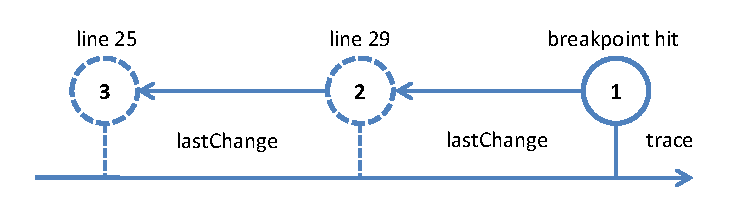
\includegraphics [width=.48\textwidth]{5-example-points.pdf} 
\caption{The examined points before locating the defect. The arrow represents the logical forward progress of the program. Three actual executions are superimposed on this arrow. All three stop at the reproduction point indicated by circle 1. After the first execution, the developer asks for lastChange as described in section \ref{sec:introExample}, yielding information  indicated by circle 2. After the second execution, another lastChange query causes a third execution, yielding information indicated by circle 3.}
\label{fig:example-points}
\end{figure}


Looking at line 29, it seems that something is wrong with
\texttt{myCondition.value} which causes line 29 execution. The
developer examines \texttt{myCondition.value} and it is
\texttt{undefined}. The next step is to know when this property got
this value. To do so, the developer runs the \textit{lastChange} command
on \texttt{myCondition.value} at this point. The debugger re-executes the
program and breaks again on line 22, analyzes its queries and shows the developer line 25-the
place \texttt{oldValue} is assigned to
\texttt{myCondition.value}. If the developer asks for \textit{lastChange} on \texttt{oldValue}, 
the debugger can notify the developer that this variable is never assigned a value.
 Now it is clear that the bug occurs because \texttt{oldValue} is
\texttt{undefined} once the execution reaches line 25 (Figure~\ref{fig:example4}).


As demonstrated in Figure~\ref{fig:example-points}, the developer has
examined three points of execution. The first point  was the breakpoint set by the developer. 
We call this special breakpoint the \textit{reproduction point}.
The second and third points preceded the reproduction point in execution sequence.
All three points-the history
of the search for the defect-are available through the debugger's
interface. On the top of the left panel in Figure~\ref{fig:example4}
there is an opened list which shows all three examined points. The
first one is the breakpoint on line 22, the second one is the point
which is when \texttt{myObject.myProperty} changed before
reaching the breakpoint and finally the last one is the point of
execution in which \texttt{myCondition.value} gets the
\texttt{undefined} value. Moreover, the source lines related to these
points are marked with red \textbf{Q} icons.

\begin{figure*}[htp]

\subfigure[A screen shot of the Firebug debugger while running the example code from Fig.~\ref{fig:js-code}. The Script
  panel is selected; it gives access to
  all loaded source files and allows breakpoints to be set on lines. In this
  figure, the execution is paused at line 22 by a regular
  breakpoint. The Watch panel on the right shows the program state at
  the paused
  point. Developer can query \textit{lastChange} on \texttt{myObject.myProperty} by right-clicking on the value of \texttt{myProperty}. ]{\label{fig:example1}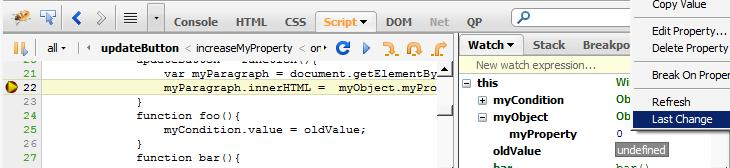
\includegraphics[width=1.0\textwidth, %height=.17\textheight
  ]{1-bp22.jpg}}


\subfigure[The result of \textit{lastChange} query for
  \texttt{myObject.myProperty}. The left panel, QP, shows the source
  code at the point of \textit{lastChange}; The right panel,
  TraceData, shows the collected data at the
  point.]{\label{fig:example3}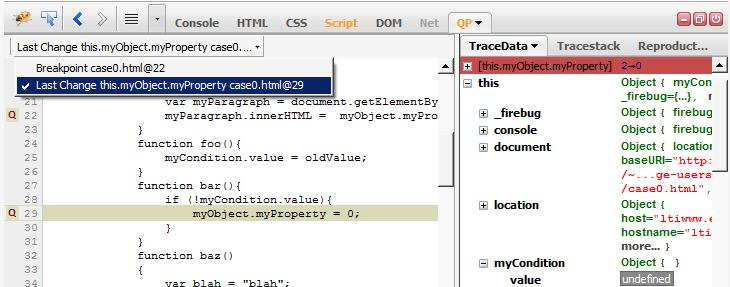
\includegraphics[width=1.0\textwidth,% height=.21\textheight
  ]{3-lastChange.jpg}}

\subfigure[The result of \textit{lastChange} query for
  \texttt{myCondition.value}. To evaluate an expression (e.g., oldValue) at this point, developer can %TODO should we remove it?
  enter the expression in the watch box and after re-execution the result is available.
  The opened list on the top of the left panel shows the visited execution points. Clicking on each point in
  the list shows the corresponding code and
  data.]{\label{fig:example4}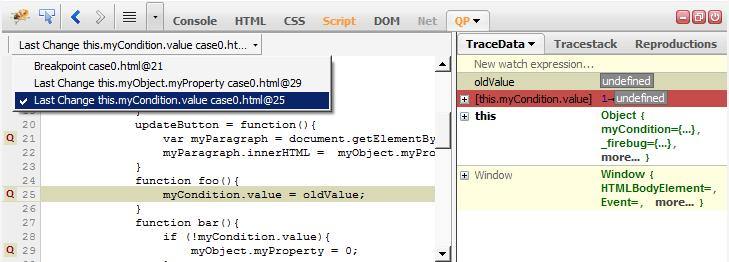
\includegraphics[width=1.0\textwidth%,height=.25\textheight
    ]{4-lastChange2.jpg}}

\caption{The stages of locating the defect using \textit{lastChange} feature.}
\label{fig:lastChange}
\end{figure*}


Notice that in our example, \textit{lastChange} combines some aspects
of breakpoint and of log-based debugging. Like breakpoint debugging,
the developer re-executes a live runtime without changing the source
and without a special execution environment beyond the debugger. The
state of the program memory and the call stack are available at each
lastChange point. Like log-based debugging, the program state and the
call stack are recorded during program execution. We can't halt the
program at \textit{lastChange} because we don't know which point is the last
one until we return to the original breakpoint. In section 5 we
discuss cases where it is possible to pause at lines of \textit{lastChange}.


\section{lastChange Algorithm}

The \textit{lastChange} algorithm is based on program re-execution of
a program halted on a breakpoint. The algorithm starts when developer
examines the program state at a breakpoint hit and asks for the
\textit{lastChange} of a value. The breakpoint hit becomes the
\textit{reproduction point}. Debugger sets hooks (a callback
function dependent upon the underlying runtime) on all instructions
that might be the result of \textit{lastChange} query. Then the
debugger re-executes the program and every time a hook hits it
checks for a \textit{change event}. In the case of a change, it stores
part of the program state values.  Once the execution reaches the
reproduction point, it analyzes the collected data and shows the
result.  The program state at the execution point of the last change
event is the \textit{lastChange}.


As we described in the preceding section, a \textit{lastChange} query can
be performed on the result of another \textit{lastChange} query. If we
name the reproduction point \textit{R}, we can write the first
\textit{lastChange} in the introductory example in this form:
\textit{lastChange(R, myObject.myProperty)}. It means that this query
is defined at \textit{R}. If we name the result of this query
\textit{L}, we can write the second \textit{lastChange} in this form:
\textit{lastChange(L, myCondition.value)}. In this way, a sequence of
\textit{lastChange} queries with any length can be defined. 

\textit{lastChange} can be called on object property, on a variable value, 
or on the results of a \textit{lastChange}. Moroever, common data structures such as
arrays and hashmaps are also supported as special cases of \textit{lastChange} on object property.
We explain each case in the following subsections.

\subsection{{\large\bf\textit{lastChange}} on Object Property}
To simplify the algorithm explanation and defer technical details, we
define two basic operations and later we explain the details of these
two operations. The first operation is \texttt{objectId()}: given a
JavaScript object it returns an integer as its identifier. This
identifier is unique to the object during one execution.  By using an
object id instead of an object reference we allow the garbage
collector to reclaim the space for dead objects just as it would in the
absence of the debugger. The second
operation is \texttt{setPropertyChangeHook()}: given a function and a
string, the function is called whenever a property changes and its
name matches the string. For example, if the string is 
\texttt{foo}, changes to \texttt{bar.foo} or \texttt{baz.foo} would
call the function.  The callback function receives a reference to the
owner of \texttt{foo}. 

To see how these functions work, suppose the developer asks for the
last change of \texttt{bar.foo} at the reproduction point in a
program. The debugger calls \texttt{setPropertyChangeHook()} with
\texttt{foo} as the property name and re-executes the
program. Whenever \texttt{foo} changes and the callback function is to
be called, debugger first calls \texttt{objectId()} on the
\texttt{foo} owner object. Then it stores this owner id, the stack
frame locations, and other state values in scope at the call point. 
Then the callback returns to continue the execution. Thus the query is not 
a breakpoint in the sense of pausing for user interaction, but breakpoint 
technology can be used to implement the query.
Whenever the execution reaches the reproduction point the debugger
looks at the history of \texttt{foo} changes and finds the last
\texttt{foo} change with the same object id as \texttt{bar} id at the
reproduction point. Figure~\ref{fig:foo-changes1} shows the list of
property \texttt{foo} change events in a hypothetical
execution. \texttt{bar} id at the reproduction point is 1010, so the
last change of \texttt{bar.foo} is the fourth column. 

\begin{figure}[htp]
\centering 
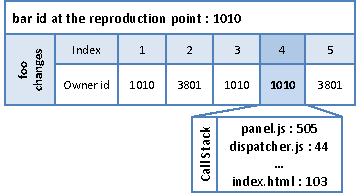
\includegraphics [width=.48\textwidth] {6-foo-changes1.pdf} %[width=.48\textwidth][scale=0.75]
\caption{A hypothetical list of  change events for a property \texttt{foo}. 
Each change event adds a column with the id of the object changed, the call stack,
and some program state such as local variable values. 
At the reproduction point  we determine which id  corresponds to 
object \texttt{bar} and read out column 4,  the last
  change of \texttt{bar.foo}. Column 3 is also a change of
  the object we want to study, id 1010, but it is not the last change;
  Column 5 is also a change of a property \texttt{foo} but it is not for
  the object we are interested in.}
\label{fig:foo-changes1}
\end{figure}

\subsection{{\large\bf\textit{lastChange}} on Variable} 
In JavaScript, every frame has a scope chain and every available
variable in the frame comes from one of the scopes in the frame's
scope chain. Once the developer asks for the last change of a variable with name 
\texttt{foo} at the reproduction point, the debugger first determines the
variable's scope as follows: it iterates over the scopes in the scope
chain and the first scope which has a variable with the same name is
the variable's scope. There are five different scope types: global, local,
closure, \texttt{with} and \texttt{catch}. We explain these
cases in two groups.

\subsubsection{global and \texttt{with} scopes}
Global scope is the most outer scope in the scope chain and it is
also referred to as the global object (the \texttt{window}
object in Web pages). This scope is a regular JavaScript object and therefore every
global variable is a property of global object. Similarly,
 \texttt{with} scopes are also regular JavaScript objects. A \texttt{with}
scope is created by a \texttt{with()} block with an object as the
parameter. Every property of this parameter object is available inside the
block as a variable. \textit{lastChange} treats the case where variable's scope
is global or \texttt{with}, like it does on an object
property.

\subsubsection{local, closure and \texttt{catch} scopes}
Local scope refers to the most nested scope in the scope
chain which contains the local variables. Closure scope refers to the 
scope which is created for a nested function and contains variables 
defined in the outer block. Catch scope is the scope created in the catch
block of try-catch statements and contains the exception
variable. These scopes are not necessarily regular JavaScript
objects.  
Therefore, to track changes to a variable in these scopes we
employ a different approach.


\begin{figure}[htp]
%\begin{verbatim}
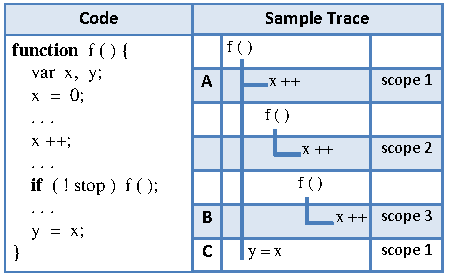
\includegraphics [width=.48\textwidth] {9-scopes.pdf} %[width=.48\textwidth][scale=0.75]


%\lstset{basicstyle=\scriptsize}
%\begin{lstlisting}[language=myLang, framerule=0pt]
%  function f(){
%    var x = 0;	
%    x++;
%    ...
%    if (!stop) f();
%  }

%Sample Trace:

%   f()
%A  |  x changes, scope 1 
%   |  f()
%   |  |  x changes, scope 2
%   |  |  f()
%B  |  |  |  x changes, scope 3 
%C  |  ... , scope 1
%\end{lstlisting}
%\end{verbatim}
\caption{A recursive call trace illustrating the scope
  id. The lines in the bottom half of the diagram simulate a trace of the change events for the variable \texttt{x} as the function \texttt{f()} calls itself. Each call creates a scope; eventually when the variable \texttt{stop} is changed by an external process we return from the recursion. The lines marked A, B, and C are discussed in the text.}
\label{fig:recursive}
\end{figure}

Having the scope chain and the source code, we can map every scope to % perhaps needs more explanation, how?
a code block, enclosed the executing code. In
JavaScript, a code block can be identified by the file url and  
the block's first instruction program counter. Given this information, the debugger is
able to recognize the code block in loaded scripts or once it is loaded.
Similar to \textit{lastChange} on object property, we define two basic operations: 
\texttt{scopeId()} -- which returns an integer given a scope -- and \texttt{setVariableChangeHook()} -- which calls its first parameter, a callback function, when a 
variable in its second parameter, a code block, matches the name given in the third parameter.

Figure~\ref{fig:recursive} illustrates how the \texttt{scopeId()} operation separates instances 
of a variable in different scopes having the same name.
If we ask for the last change on \texttt{x} at point labeled \texttt{C} in scope with id 1, we want the change at line \texttt{A} in scope 1, not 
the change at the line marked \texttt{B}, where a variable named \texttt{x} in scope 3 is changed.  


If the developer asks for the last change of variable \texttt{foo} at the 
reproduction point in a program, debugger calls 
\texttt{setVari- ableChangeHook()} with the variable's defining
block and name as parameters and re-executes the
program. Whenever \texttt{foo} changes and the callback function is to
be called, debugger first calls \texttt{scopeId()} on the
variable's scope. Then it stores this scope id, the stack
frame locations, and other state values in scope at the call point.
Whenever the execution reaches the reproduction point the debugger
looks at the history of \texttt{foo} changes and finds the last
\texttt{foo} change with the same scope id as the variable's scope id
at the reproduction point (Figure~\ref{fig:foo-changes2}). 

\begin{figure}[htp]
\centering 
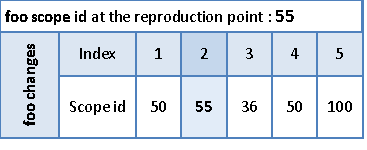
\includegraphics[width=.40\textwidth]{7-foo-changes2.pdf}
\caption{A hypothetical list of variable \texttt{foo} change events. Each column of the list indicates a change event; for each
change event the scope id returns by \texttt{scopeId()} is recorded along with call stack and program state information. 
   The last column having the scope id \texttt{foo} at the reproduction point indicates 
  the last change.}
\label{fig:foo-changes2}
\end{figure}


\subsection{{\large\bf\textit{lastChange}} on {\large\bf\textit{lastChange}}}
The \textit{lastChange} algorithm records changes by id (either object or scope id), then reads out the last change when we
arrive at the reproduction point and discover the id of the requested value.
When we perform \textit{lastChange} based on a previous \textit{lastChange}, the query algorithm 
must retain additional information. Consider the following example:

\lstdefinelanguage{myLang2}
{morekeywords={point, lastChange}}

\lstset{basicstyle=\small}
\begin{lstlisting}[frame=single, language=myLang2] %, framerule=0pt]

 point A : the reproduction point 
 point B : lastChange(A, bar.x) 
 point C : lastChange(B, baz.y) 
\end{lstlisting}

%\begin{center}
%\textit{
% }
% \end{center}

where point A is a breakpoint, point B is the last change of the object property \texttt{bar.x} at point A, and
point C is the last change of the object property \texttt{baz.y} at point B. 
The object referenced by \texttt{baz} changes upon re-execution. Therefore when the developer
asks for the last change of \texttt{baz.y}, we need to track objects named \texttt{baz}
at changes of \texttt{bar.x} and changes to objects named \texttt{y}. Then, at the reproduction point,
we need to work out which \texttt{baz} the developer wanted, then select the last change of that \texttt{baz.y}.
Figure~\ref{fig:lastchange-lastchange} illustrates the extra row of data (tracking of \texttt{baz} objects 
at \texttt{x} change events) 
and how the id values allow the last change of \texttt{baz.y} to be worked out. 
 
In the general case we perform dependency analysis as outlined in 
Figure~\ref{fig:dependency-analysis} to
create the list of additional data (object id or scope id) to be collected at a change
event. The process can be repeated to cascade \textit{lastChange} arbitrarily deep.


\begin{figure}[htp]
\centering 
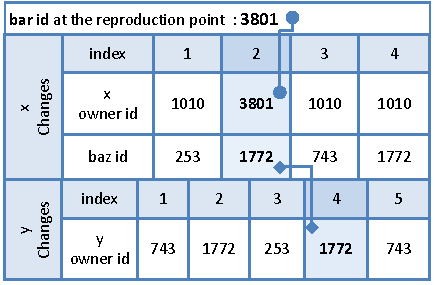
\includegraphics[width=.48\textwidth]{8-lastchange-lastchange.pdf}
\caption{The list of change events stored for locating point B, the
  \textit{lastChange} of \texttt{bar.x} at the reproduction point, and
  point C, the \textit{lastChange} of \texttt{baz.y} at point B.}
\label{fig:lastchange-lastchange}
\end{figure}



\begin{figure}[htp]
%\centering 
%\begin{algorithm}
\line(1,0){240}
\begin{algorithmic}%[frame=single]
\FOR{$q$ in $lastChange$ queries} 
 \FOR {$p$ is defined at the $q$ result}
   \IF {$p$ is a $lastChange$ on object property} 
     \STATE the property {\bf owner id} must be stored at $q$ change events. 
   \ELSIF {$p$ is a $lastChange$ on variable} 
     \STATE the variable {\bf scope id} must be stored at $q$ change events.
	 \ENDIF 
 \ENDFOR 
\ENDFOR

\end{algorithmic}
\line(1,0){240}
%\end{algorithm}
\caption{\textit{lastChange} queries dependency analysis.}
\label{fig:dependency-analysis}
\end{figure}
%---------------------------------------------------------------------------------------------------
\section{JavaScript implementation}
To verify the \textit{lastChange} algorithm we
implemented\footnote[1]{http://code.google.com/p/querypoint-debugging} it in an extension to the Firebug
JavaScript debugger\footnote[2]{http://getfirebug.com}. %\cite{Firebug}. %\cite{firebug-version-1.6}. 
Firebug itself is an extension of the Firefox browser. %\cite{Firefox}. %\cite{firefox-version-3.6}
The Firefox JavaScript engine provides a JavaScript debugging interface \cite{JSD} and 
\textit{Querypoint} is developed over this interface. Our prototype implements the four primitive operations in JavaScript 
using techniques which are cumbersome and comparatively slow to execute. However the JavaScript prototype is
easy to explore, change, and share with others for feedback. A professionally useful debugger 
would implement these primitive operations within the JavaScript engine.


\subsection{{\normalsize\bf\texttt{objectId()}} Operation}
\texttt{objectId(obj)} first checks the argument \texttt{obj} for a property \texttt{\_objectId}.
%\footnote[3]{The property name we used in the prototype is longer and more specific to reduce the chance of name conflicts.} .
It returns the value if this property is already defined,
otherwise it generates a new id and sets this property. The value of the id is simply an integer incremented 
for each new \texttt{\_objectId} needed. 
%\footnote[3]{This use of a regular object property  might change
%the program behaviour. For example it will appear as an extra property in 
%\texttt{for(property in object)} loops. 
%The next version of Firefox (https://developer.mozilla.org/en/JavaScript/Reference\\/Global\_Objects/Object/defineProperty) provides \texttt{defineProperty}, 
%allowing a property to be added which is invisible to enumeration.} Note that \texttt{\_objectId} is
%not set for all objects but only those objects that need an id.



\subsection{{\normalsize\bf\texttt{setPropertyChangeHook()}} Operation}
The Firefox JavaScript engine supports watching property changes in an
object. Every object has a function \texttt{watch(propName, callback)}
which receives two parameters, a property name and a function.  Whenever
the property with the given name changes, the \texttt{callback} function is
called. The hook set by this function remains enabled even if the
property is deleted and defined again. 

For our purposes, the \texttt{watch()} function only covers the case
of global object properties. At the beginning of execution, no object
excepting the global object and its predefined properties is available.  For 
our \textit{lastChange} prototype, we created a version of
\texttt{setPropertyChangeHook()}.  The basic strategy is to get a reference to the object just
after its creation, then use \texttt{watch()} function to monitor
property changes in the object. Setting a flag\footnote[3]{DISABLE\_OBJECT\_TRACE defined in jsdIDebuggerService.idl} into the Firefox 
JavaScript engine, we can get the file URL and the line number for each object
creation (e.g., myFile.js, line 24). We set a breakpoint on this line
and parse the source code to determine which object was created.

The only data we have is the object creation location including the
file url and the line number and the goal is to get a reference to
this object. Although in most regular cases we have only one
statement and one object creation, there are cases where more
objects are created in the line. There is no simple way to
recognize the interesting object among these new objects. So instead
of one object, we monitor all new objects created in the line.

An object might be created by one of these statements: object
literal(\texttt{\{...\}}), \textit{new} operator (\texttt{new 
constructor()}) or function definition statement (\texttt{function()}). 
By parsing the source code we can recognize the statements that
create an object. The next step is getting a reference to the new object.

The new object can be assigned to an object property or a variable by
an assignment (\texttt{=}). In these cases we keep the assignee statement 
at the left side. The idea is that we create a list of assignee statements 
that the new objects are assigned to. We set a hook on the creation
line. Once the hook hits, we evaluate the assignee statements. Then 
we do stepping(step-over) and after each step we evaluate the
statements. Every statement which has a new value, we consider the new
value (if it is an object) as a new object. For example in Figure
~\ref{fig:objectCreation}(a), if the creation line number is 20, we
have only one statement which creates a new object and it is assigned
to \texttt{x.y}.

The new object can also be set as the property of a parent object 
(or array) inside an object (or array) literal. This case is also treated 
similar to previous case. The only difference is that the full path of property 
from the root parent in the local scope must be considered as the assignee statement. For
example in Figure~\ref{fig:objectCreation}(b), if the creation line
is 20, we keep \texttt{parent.child}. In this case stepping
must be continued until the end of the object literal (line 22) for getting a reference
to the created new object.

In cases where the new object is passed as an 
argument to a function (Figure~\ref{fig:objectCreation}(c)), we use step-in instead of step-over. 
To get a reference to the new object
it is enough to evaluate the corresponding argument inside the function. The other cases
where the program does not keep a reference to the created object (e.g., when a function object is
just called after its creation), are not in our interest. 

%(or \texttt{this} if the object is being constructed by \texttt{new} statement)

Although this approach is successful in many ordinary cases, we can imagine 
cases where a more comprehensive analysis needed for the correct behaviour. 
Consider the case where the new object is assigned to an expression like \texttt{a[++i]}. 
% (where i is a variable). 
%This expression is kept in the list                      %(Figure~\ref{fig:objectCreation}(d))
%of assignee statements to be evaluated later for getting a reference to the new object. 
Obviously, evaluating this statement doesn't return
a reference to the new object. Our prototype implementation does not handle these kinds of unusual cases yet.

Throughout this section we implicitly assumed that the object will be created at 
the same location in the next execution. If the assumption is
not true, once the execution reaches the reproduction point, it
reveals that the object has been created in a different location. This time,
prototype re-executes the program considering both locations as possible 
object creation locations.

\begin{figure}[htp]
%\begin{verbatim}
\lstset{basicstyle=\scriptsize}
\begin{lstlisting}[frame=single, language=myLang]% framerule=0pt]

(a) Case 1:
 20  x.y = new MyClass();

(b) Case 2:
 19  parent = {
 20    child : {
 21      x : 5
 22  }}

(c) Case 3:
 20  myFunction({myProperty:5});

\end{lstlisting} 

%(d) Case 4:
% 20 a[++i] = new myConstructor();

%\end{verbatim}
\caption{Examples of different cases in getting references to created JavaScript objects.}
\label{fig:objectCreation}
\end{figure}

\subsection{{\normalsize\bf\texttt{scopeId()}} Operation}
The prototype sets a breakpoint at the beginning of all code blocks needing
a scope id. The scope id is kept as a variable with name 
\texttt{\_scopeId} in the scope. Whenever the hook is hit,  meaning a new scope
is created, \texttt{\_scopeId} is set by calling JavaScript's dynamic compilation 
function \texttt{eval()}. For example, executing \texttt{eval("var \_scopeId = 10")} creates a
variable with name \texttt{\_scopeId} and value \texttt{10} in the
scope of the \texttt{eval()} call, which is our interesting scope. \texttt{scopeId()}
operation returns the value of \texttt{\_scopeId} in the scope.

\subsection{{\normalsize\bf\texttt{setVariableChangeHook()}} Operation}
Variables defined in local, closure, and catch scopes are only changed in
their scope; that includes the defining scope and scopes nested whithin them.
For example in Figure~\ref{fig:js-closure}, variable \texttt{foo} in line 11 can only be
changed in lines 10 to 23. Therefore, after locating the function in
which the variable is defined, it is enough to parse the code inside
the function block and set a hook on all lines where the variable is
assigned a new value. 
We also set a hook at the first line of the function which is
corresponding to the line where the variable is defined. In Figure~\ref{fig:js-closure}, 
if the execution is paused at line 17 and the
last change of \texttt{foo} is queried, two hooks on lines 16 and 17
will be set, but if the execution is paused at line 20 , four hooks on
lines 11, 12, 14, 20 will be set. These two cases are different: \texttt{foo} in 
\texttt{childOne} is a local variable
but in \texttt{childTwo} it is a closure variable.

\begin{figure}[htp]
%\begin{verbatim}
\lstset{basicstyle=\scriptsize}
\begin{lstlisting}[frame=single, language=myLang]%, framerule=0pt]

10  function main(){
11    var foo;
12    foo = ...;
13    function parent(){
14      foo = ...;
15      function childOne(){
16        var foo;
17        foo = ...;
18      }  
19      function childTwo(){
20        foo = ...;			      
21      }
22    }  
23  }    
\end{lstlisting}
%\end{verbatim}
\caption{Sample JavaScript code demonstrating local and closure variables.}
\label{fig:js-closure}
\end{figure}

\subsection{Re-Execution, Reproduction Point and Data Collection}
\textit{Querypoint} needs a test case to reproduce the
execution and conditions to correctly recognize the reproduction point. 
Although both elements can be directly provided by developer, \textit{Querypoint}
is also able to automatically create them from the first execution. 

To replay execution, \textit{Querypoint} keeps track of breakpoint hits and single steps. For example, 
if the developer queries \textit{lastChange} at the third hit of breakpoint \textit{b}, in
re-execution, the third hit is recognized as the reproduction point. 

The \textit{Querypoint} prototype supports two mechanism
for automatic re-execution: callstack-reproduction and record-replay. In callstack reproduction the function from
the earliest frame of the call stack is called with the same parameters. The idea
behind this mechanism is that many bugs in web pages can be reproduced by re-firing
an event like clicking on a button. The record-replay execution uses two phases. In the record phase, it 
stores the initial page url and the events and parameters corresponding to user actions. In the replay phase, it opens
the same url and simulates events as if they were user actions. The callstack reproduction mechanism provides
shorter re-execution cycles while the record-replay is more accurate about the
initial state.

In addition to the data collected at every change event for identifying the \textit{lastChange}
result, \textit{Querypoint} partially stores values in program state. There is a trade-off between the amount of data collected at every change event and the number of re-executions. If developer asks for 
some values which have not been stored, \textit{Querypoint} re-executes and collects the requested data. 


% Discuss what happens when assumptions changes, like object creation location.

\section{Reproducible Non-Deterministic Execution}
We claim that the only prerequisite for \textit{lastChange}  is bug-reproducibility. 
A bug is \textit{reproducible} for a developer when the developer can
start from a given initial state, operate on the program with a
list of actions, and reproduce the symptoms of the bug. The details of
the execution can change each time we re-execute the buggy program,
but the buggy result is the same.  All modern debuggers in wide use that we know 
about rely on reproducible but non-deterministic execution for simple practical reasons: 
developers must reproduce a bug to study it and modern execution environments 
are not deterministic.  
% In this section we discuss non-determinism and \textit{lastChange}. However we want 
%to emphasize that when developers have to think about non-determistic execution 
%it usually means that bugs are not reproducible. 
%The reproducibility of the bug
%means that the defect is very unlikely to depend on the order of
%events during the execution. Conversely, if the defect depends on the order of execution, 
%it will likely fail to reproduce on some executions. 
By relying on reproducibility but 
not requiring deterministic execution, \textit{lastChange} works on the same range of cases.

\subsection{{\large\bf\textit{lastChange}} Result Consistency}
\label{sec:resultConsistency}

Each time we re-execute a non-deterministic program, 
the details of execution instruction order may change. 
For example, if we record the source code lines every time
a conventional watchpoint hits, the record may differ each time we
re-execute. But \textit{lastChange} does not compare values across 
executions. Rather it analyzes all of the
change events in a single execution. 
Neither the data gathering nor the analysis require deterministic execution.

Since we don't need to compare values across executions to implement \textit{lastChange}, we can get more information if we do compare:
 different points of last change on different executions will signal that the execution is not deterministic. Note the converse is not true, many non-deterministic 
programs will give identical results for \textit{lastChange}.
Consider the example in Figure~\ref{fig:nondeterministic-values}. 
Assume that at the first execution, the developer sees that the \texttt{a} value is \texttt{true} and asks
for the \textit{lastChange} of \texttt{a} at the breakpoint. In the re-execution, \texttt{a} is \texttt{false},
and \texttt{b} is \texttt{true} at the reproduction point. It means that \texttt{lastChange}
result shows line 10, which is a correct answer for this execution but not for the previous one.
When user asks for the \textit{lastChange} on variable \texttt{a}, debugger stores \texttt{a} value and compares
it to the \texttt{a} value in the next executions. So if this value is different, debugger informs the developer
that the \textit{lastChange} query is made on a different value.
% In cases that the value is not a primitive but an object,
%the primitive properties of the object examined by the developer are stored and compared.

\begin{figure}[htp]
%\begin{verbatim}
\lstset{basicstyle=\scriptsize}
\begin{lstlisting}[frame=single, language=myLang]%, framerule=0pt]

10 a = b = false;
20 if (random()) {a = true;} else {b = true;}
30 if (a || b) {bug(); /* breakpoint */}
\end{lstlisting}
%\end{verbatim}
\caption{\textit{lastChange} on non-deterministic values.}
\label{fig:nondeterministic-values}
\end{figure}

\subsection{Combination of {\large\bf\textit{lastChange}} and Breakpoint Debugging}
\label{sec:pausing}
Using \textit{lastChange} a developer can work backwards on the flow of data, but sometimes bugs are more obvious when
we watch control flow forwards. Consider for example, 

%\begin{verbatim}
\lstset{basicstyle=\scriptsize}
\begin{lstlisting}[frame=single, language=myLang] % framerule=0pt]

44 vector.r = Math.floor(Math.random()*5)*6;
45 if (vector.r !== 0 && vector.r < 30);
46   return vector;
\end{lstlisting}
%\end{verbatim}
where \textit{lastChange} shows us that \texttt{vector.r} is zero at line 44. In our user studies, developers
wanted to single step forward from line 44. If they could do this, they may be surprised to see line 46 execute 
even if \texttt{vector.r} is zero, directing their attention to line 45 where they can discover the errant semicolon.
However, a \textit{lastChange} is just a query result, not a breakpoint. Under what conditions can we 
cause the debugger to stop at the \textit{lastChange} point?

In the case that the execution is deterministic, the \textit{last-\ Change}
event index can be used as an index for a conditional breakpoint \cite{Boothe, Maruyama}. 
Moreover, this works in a non-deterministic execution if non-determinism
has no effect on the event index.  The debugger can easily set this conditional breakpoint
and reexecute the program. If the stream of change events differs in this re-execution the
developer can be warned that the conditional breakpoint may not be the \textit{lastChange} point.
However, if the stream of events is the same, we do not know that the 
conditional breakpoint matches the last 
change, this fact can only be verified at the reproduction point. These theoretical concerns are not
likely to cause significant practical problems: if the value at the conditional breakpoint is not suspicious, 
then the developer will know to simply return to \textit{lastChange} or move on to another tactic to find the bug.

% Cut to reduce size
%There are cases where event indexes fail, but a developer can use knowledge gained from \textit{lastChange}
%to formulate a conditional breakpoint.
%Consider the example in Figure~\ref{fig:counter-example}. It shows a function which processes an
%array. The array contains numbers except one item which is
%\texttt{undefined} and it causes a bug in line 30. There is a call to
%\texttt{randomPermutation} function in line 11 which randomly
%permutes the array item. So at every execution the
%\texttt{undefined} item will be in a new place. Calling
%\textit{lastChange} on \texttt{x} at the place the bug happens, gives a
%point which shows line 14. Although this point exists at every
%re-execution but it can not be identified by an event index. A conditional breakpoint on 
%the value of the item would succeed and the developer can reason from the 
%textit{lastChange} results to create the condition. 

%\begin{figure}[htp]
%\lstset{basicstyle=\scriptsize}
%\begin{lstlisting}[language=myLang, framerule=0pt]
%10 function randomProcess(array){
%11   randomPermutation(array);
%12   var x, y;
%13   for (var i=0 ; i<array.length ; i++){
%14      x = array[i]
%...
%30      y = x+1;
%31   }
%32 }
%\end{lstlisting}
%\caption{A counter-example for transforming \textit{lastChange} to a conditional breakpoint.}
%\label{fig:counter-example}
%\end{figure}


\section{User Study}
We supplied four experienced Javascript developers with our prototype in an 
extended Firebug debugger\footnote[4]{http://ltiwww.epfl.ch/\texttildelow mirghase/lastchange-userstudy}. Following a tutorial and a practice case, we observed as they 
applied both conventional breakpoint and \textit{lastChange} on two small programs we 
provided (Our prototype did not have a user interface to support Sec.~\ref{sec:pausing}).
The first program, Shapes, calculates the area and perimeter values for a list of shapes. The bug happens when one of the calculated numbers is zero. The second program, Moving Circle, randomly scales and moves a circle in the page. The bug happens once the circle becomes invisible after an exception
occurs. This case represent a reproducible non-deterministic execution. The developers were asked to locate the defects that caused these bugs. All four developers successfully applied \textit{lastChange} to the test programs 
and understood how it could help debugging. 

To find the defect location with breakpoints, all four users took more steps and more time (Figure~\ref{fig:userstudy}).  
Two users scrolled through the source, 
another searched the text, a third set a lot of breakpoints to understand the control flow. 
Based on our own experience we expect these strategies represent the kinds of approaches 
developers have available. These operations are time consuming and tedious. In contrast, all four users 
found the defect location with just two \textit{lastChange} operations.
% Based on our measurements,
%this makes \textit{lastChange} about three times faster than breakpoints for the navigation from 
%the reproduction point to the defect
We recognize that these programs were designed to highlight lastChange and many kinds of debugging 
issues have been hidden by the design of our tests. Nevertheless our results show that, when a defect 
relates to incorrect values and a developer recognizes this, then the operational 
mechanics of lastChange lead to the defect much more quickly than breakpoints.

Our observation and discussions with users also brought out several important issues and improvements
for our user interface. Perhaps the most important and challenging improvement would be better integration 
with breakpoint debugging. Our implementation put the results of \textit{lastChange} in a similar but different
view from breakpoint debugging. This focuses attention on value changes, but it makes studying control 
flow more difficult: we don't support single stepping from a \textit{lastChange} result in our user interface. In our next iteration we 
plan to merge the query and breakpoint results and support pausing as described in Sec.~\ref{sec:pausing}.


\begin{figure}[htp]
\centering 
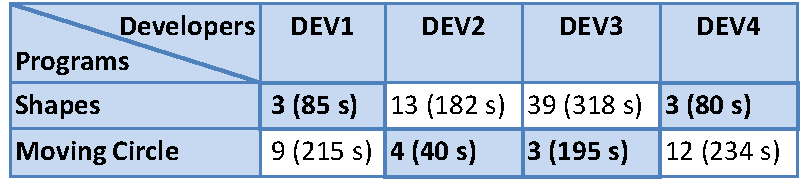
\includegraphics[width=.48\textwidth]{10-userstudy.pdf}
\caption{The number of steps (and time in seconds) required before locating a defect, for each test subject and test program. 
Cells with a white background report values with conventional debugging; Cells with a colored background use \textit{lastChange}.}

\label{fig:userstudy}
\end{figure}

\section{Discussion}

We have presented the \textit{lastChange} algorithm and described our
prototype implementation. Our goal is practical improvements in debugging. To achieve our goal we need practical JavaScript engines
to add new debug primitives so that developers in the field can use our new technique. This paper is
one step to convince implementers to enable \textit{lastChange}.
Thus we summarize here our arguments that \textit{lastChange} should be supported.

%The key ingredients in our argument are: 
%\begin{enumerate}
%   \item developers need an operation like \textit{lastChange}, 
%   \item developers can learn to use \textit{lastChange}, 
%   \item practical implementations are feasible with modest
%invested development time,
%   \item in most cases \textit{lastChange} will be much faster than current alternatives,
%   \item the worst cases are not more common or more painful than
%alternatives.
%	 \item the \textit{lastChange} approach can be generalized to other queries.
%\end{enumerate}

%TODOWe have also developed a prototype implementation of the debugger control part of lastChange for Java. The main differences (one or two sentences). We will report on this implementation in a later publication
\subsection{Developers need an operation like \protect{\large\bf\textit{last- Change}} }

%We have shown how \textit{lastChange} identifies the prior point in
%program execution where a program state value changes. Is it something
%the developer needs to do?  

Since ultimately programs are just
transformation of state values, debugging is ultimately backtracking
to find defects in program state change\cite{Weiser,Zeller}.  When a developer halts a
program on a breakpoint they compare the call stack and program state to their model of the program.
If any value seems to be incorrect,  they need to figure out what operation
causes the incorrect value. Here \textit{lastChange} takes over and addresses a key
part of the debugging process.
%have three kinds of information: a model
%of the program in their mind, a call stack showing what part of the
%program is halted, and the state at that point (a combination of the
%debugger's view of the program internal state and the output of the
%program up to this point of execution). If the model does not match
%the call stack or if no value in the viewable program state aligns
%with the developers model for this point in execution, the developer
%will seek another view by changing the breakpoint or the input
%data. If a value appears incorrect, they may have a flash of insight
%and know the defect. Otherwise they need to figure out what operation
%causes the incorrect value. Here \textit{lastChange} takes over and addresses a key
%part of the debugging process.

\subsection{Developers can learn to use \protect{\large\bf\textit{lastChange}}}

%If \texttt{lastChange} could be useful, can developers figure out how
%to use it? 
While our user study was small, our prototype demonstrates that
\textit{lastChange} can be easily activated by operations on the
graphical representation of erroneous data in a debugger and the 
results can be interpreted by users. 
While \textit{lastChange} is not a breakpoint, 
all of the assumptions developers already have for breakpoints hold
for \textit{lastChange}. In particular the re-execution is just the
same operation developers use to debug with breakpoints. 

%We designed the
%user interface for the results from \textit{lastChange} to resemble
%the results from a breakpoint, with the source code of the change
%point highlighted and the state of the program presented the way state
%is presented from a breakpoint. Based on this user interface, we
%believe developers can start to use \textit{lastChange} with minimal
%training. Our users may not be representative, but the key point here
%is that the learning curve is small compared with the challenge of learning 
%breakpoint debugging in the first place.

%In our own experience, \textit{lastChange} dramatically reduces the work in
%setting and removing breakpoints, so work to cause re-execution  become noticeable.
%Therefore automatic mechanisms
%for re-execution will be corresponding more valuable for debugging
%with \textit{lastChange} (Our \textit{Querypoint} prototype  
%implements a simple form of automatic 
%re-execution for both breakpoint and \textit{lastChange}).


\subsection{Practical implementations are feasible}

We have described our prototype all-JavaScript implementation in Sec. 4. It is adequate for 
exploring the ideas and may even be usable in production. However significant 
improvments can be made. A fully usable
implementation would require access to the object id at the point of
object creation and \texttt{setPropertyChangeHook()}. Many
object-oriented runtimes provide object identifiers and 
provide access to object creation directly or by bytecode instrumentation\cite{JPDA}. 
%In the particular case of the Firefox Web browser we used for our prototype, the primary barrier
%to practical implementation would likely be integration with the
%increasingly sophisticated just in time compilers. In the case of
%tracking variable changes, \texttt{setVariableChangeHook()} can be implemented
%similar to \texttt{setPropertyChangeHook()} if JavaScript scopes-like regular 
%JavaScript objects-support \texttt{watch()} function.

\subsection{In most cases \protect{\large\bf\textit{lastChange}} will be much faster than current alternatives}

%When developers try \textit{lastChange}, will they get results fast
%enough to benefit? While we only used our prototype on toy programs,
%\textit{lastChange} seemed as fast as breakpoint re-execution.
%But what can we say about realistic programs?

Recall that we
insert additional code through debugger callbacks, then re-execute the
program. The additional code we insert is proportional (in our
JavaScript algorithm) to 1) the number of places a property or
variable with a given name is changed, 2) the number of places objects
are created. The overhead for each execution at a change event
 depends upon the amount of data we store for each change event; 
the overhead for object creation could be small since we only need to 
determine if the object is one we need to watch.  

%We implemented a
%simple and effective mechanism allowing developers to control 
%overhead: we stored data to a depth of two property accesses 
%(e.g. foo.bar.x), then placed a \textit{re-run} button 
%in the user interface at the third level. If developers reached the 
%third level they can see more data at the cost of one more replay.

For comparison consider today's practical alternative: developers
setting breakpoints. For the vast majority of programs, a developer
will take much more time to set one breakpoint than
\textit{lastChange} would add. Moreover, typically the developer may not
guess the point of last change. They must then ponder another
breakpoint and re-execute. 

%Unlike the re-execution we use to 
%optimize performance in \textit{lastChange}, 
%developers still will not know if the breakpoint they hit is the point of last change
 %or even if it is related to the change at all.

We could also compare to solutions based on logging or tracing. Manual
logging has very high overhead: the developer must add code, debug
that added code, then analyze the log (To be fair, the log can become
a permanent debugging aid). Automatic logging as we discuss in 
section \ref{sec:relatedWork} causes about one or two orders of magnitude slow down as well
as requiring a completely different set of development tools. 

\subsection{The worst cases are not more common or more painful than alternatives}

%Finally we consider the worst cases: what about code that changes
%objects in long running loops? 
Every time through the loop we incur
the call back overhead; if the loop itself has relatively little code
the overhead could be very large; if the loop computation is a
significant fraction of the full program, the slowdown would be
enormous. 
Other techniques also struggle with this case:  breakpoints in highly repeating loops are not feasible and logging
becomes unwieldy. 
Developers face this issue with any debugger today: occasionally a
debugger causes too much overhead to be useful for debugging. 
%Since automatic logging solutions are highly tuned,
%their overhead in this case will likely be much less than
%\textit{lastChange}. On the other hand, \textit{lastChange} integrates
%with an interactive debugger and detecting that we are in a high
%overhead loop is simply a matter of checking our internal counter. %
%In
%such unusual cases we may simply offer the developer the option of
%studying the loop code then omitting it from \textit{lastChange}
%operations. 
%
%The users of \textit{lastChange} may encounter these kinds of cases, but 
%that is the nature of debugging: you need different tools for 
%different kinds of problems.

\subsection{Generalizations}
Our \textit{lastChange} algorithm can be viewed as a particular interface to a general facility. 
The general facility replays execution, queries the runtime at points of interest during execution,
and analyzes the result at the reproduction point. We have selected one kind of query and analysis
that can be easily integrated in existing debuggers and explained to developers, providing automation of 
the problem of finding the point of last change. We believe other
kinds of queries and analysis can be invented and integrated to automate other aspects of debugging.
%Moreover, the query history analysis used to test for non-determinism here may also be the basis for
%more effective user interfaces to debugging sessions. The series of cascaded \textit{lastChange} queries becomes 
%logical path followed by the developer seeking the defect and this path may be useful if presented in effective user interfaces.

\section{Related Work}
\label{sec:relatedWork}
%The algorithm we presented in this paper obtain information about
%the execution state logically earlier in the control flow by querying 
%the executioin state during replay using the technology of 
%conventional breakpoint debuggers.  
The \textit{lastChange} approach resembles the operational model of replay-based debugging 
and the query approach of logging-based
debugging.  Replay-based approaches capture limited data during
execution and replay the buggy execution to reach past points. In
contrast, logging-based approaches collect enough data during
execution to relieve developer from re-execution, then query the data to 
inform the developer. Replay-based
approaches impose much less runtime overhead (about two orders of
magnitudes) comparing to logging-based approaches. However, developer
has to re-execute the buggy execution several
times. \textit{lastChange} collects data on re-execution by queries
selected by developer interaction with the debugger. Therefore it has 
the selectivity of the replay-based approaches that improves performance, 
% but we have 
and the flexibilty of the queries so it does not require deterministic replay.

Among replay-based debuggers we compare to bdb \cite{Boothe} and
reverse watchpoint \cite{Maruyama}.  A bidirectional C debugger, bdb
employs a step counter to locate the requested point from the
beginning of execution. It relies on deterministic execution replay
%(i.e., the same sequence of instructions in re-execution) 
and records the results of non-deterministic system calls and re-injects them into
the program when it is replayed. It makes use of checkpoints to reduce
the time needed for re-execution. Reverse watchpoint, similar to bdb, uses
a counter to correctly locate the last write access of a selected variable in the
next execution \cite{Maruyama}.
% Reverse watchpoint is proposed by Maruyama et al., analyses the execution and moves the debugger to the
% last write access of a selected variable by re-executing the program
%from the beginning\cite{Maruyama}.  Similar to bdb it relies on deterministic
%replay and uses a counter to correctly locate a point in the next
%execution. 
The main disadvantage of these approaches is that they require 
identical, instruction by instruction, re-executions. % exactly the same executions. 
Even one instruction difference between
two executions leads to wrong results. On the other hand,
\textit{lastChange} doesn't require any special feature in the
re-execution and fits into existing debugging practice

Among logging-based approaches are \textit{omniscient} debuggers
ODB\cite{Lewis} and Unstuck\cite{Hofer}. Both
approaches keep the log history in memory and hence can only record
and store the complete history for a short period of time. These
debuggers record all the events that occur during the buggy execution
and later let the developer to navigate through the obtained execution
log. In these approaches there is no execution to resume: moving
backwards in the log can be similar to moving forwards. A more scalable 
approach to omniscient debugging has been proposed by Pothier et al. \cite{Pothier}. 
Their back-in-time debugger, TOD, addresses the space problem by storing 
execution events in a distributed database. Bhansali et al. \cite{Bhansali} attempted to address the performance overhead 
and large trace size of logging-based debugging in their time-travelling debugger, Nirvana. 
Nirvana first collects a full compressed trace of program execution and then 
simulates re-execution. Their results are quite similar to omniscient 
debuggers. Nirvana incurs about 15 to 68 times runtime overhead in 
re-simulation.


Logging-based debuggers suffer from different issues. First, the recording
step is time expensive and it should be repeated in case of changes in
program. Second, the execution log cannot fully replace the live
execution. There are other aspects of execution (e.g., program user
interface, file system, database tables, etc.) which are also
important in debugging and are not available to the developer in
omniscient debuggers. Third, querying collected data (e.g., to restore
the program state at a certain point) may not be efficient enough for
debugging realistic programs. Comparing to logging-based debuggers our approach is 
has little upfront cost and more flexibility. The developer can start debugging just 
after reproducing bug without a capturing step.  Changing inputs or
environment settings and re-executing to investigate the bug works as
in conventional breakpoint debuggers.


Program slicing\cite{Weiser} approaches debugging from a completely different perspective. Given a point of interest {\bf S} in a program, a \textit{slice} is an executable subset of the program affecting {\bf S}.  Many studies have shown ways to compute the slice more quickly or to constrain the slice to a smaller subset of the program \cite{Horwitz, Sridharan}.  Dynamic slicing \cite{Korel} applies slicing analysis at run time and thus most closely resembles \textit{lastChange} from among the slicing approaches.  Our \textit{lastChange} approach can be related this way: first, allow the developer to select from {\bf S} a key critical value {\bf V}. Then compute a slice affecting {\bf V}. Show the developer only the most relevant part of that slice (the \textit{lastChange}). Finally iterate towards the fault by chaining new slice-selection criteria.

Both approaches rely on selecting {\bf S}. Both approaches differ from breakpoint debugging in analyzing a program from a known good point (e.g. start of the program) to {\bf S}. Slicing reduces the space the developer needs to search, but provides no guidance within the slice; \textit{lastChange} explores the slice using developer-selected search criteria, but does not help the developer recognize code that cannot impact {\bf S}. Slicing requires a sophisticated compiler-like technology while \textit{lastChange} builds on familiar run-time debugger technology. 

A recent work by Lienhard et al.\cite{Lienhard} suggests virtual
machine level support for keeping the history of events. It replaces every
object reference with an alias object which keeps the history of
changes to the object reference. 
%In this way, when an object is
%collected by garbage collector, its track of changes (if it is not
%referenced by other aliases) will be also collected. 
Although this approach incurs less runtime overhead (7 times) in
comparison to omniscient debuggers, it adds memory
overhead. 

Origin tracking of \texttt{undefined} and \texttt{null} values employing \textit{value piggybacking} technique proposed by
Bond et al. \cite{Bond}. This approach has two main limitations comparing to \textit{lastChange}.
First, it is limited to \texttt{undefined} and \texttt{null} values. Second, it does not return the last change
of a \texttt{null} variable but the first place that the \texttt{null} value is originated.


%Two new directions in logging debuggers explore more detailed use of
%the log and more effective user interface to the collected data. %logging approaches. 
%WhyLine\cite{Ko} provides visual interface to collected runtime information and lets
%developer moves on execution log using queries expressed in terms of
%the programming objects. 

WhyLine\cite{Ko} stores the program user interface in
addition to the program trace and provides answers to why and why not
questions to the user. 
%Jive\cite{Czyz} depicts the history of
%execution by a sequence diagram and lets the user to query on the events
%database. 
WhyLine suffers from the requirement of gathering tracing information before its unique capabilities can be used.
We imagine that the runtime queries we use in \textit{lastChange} may be used to gather data incrementally for this kind of debugging approach.

%Querypoint debugging uses re-executions to gather infor-mation requested by the developer: the memory overhead depends on the query not the entire program. Moreover, the Lienhard et al. debugger significantly changes the virtual machine, while our approach is a generalization to conditional breakpoints and available debugger infrastructure can be adapted to support it.
 
%\textit{lastChange} functionality does rely on a conventional breakpoint to begin queries, a requirement not shared by full logging solutions.  Here we leverage past experience of developers, but there are also new tools [] to help with this problem in the case of graphical and event based systems.


\section{Conclusion}
\textit{lastChange} provides critical information for debugging programs: the location and state at the point where a questionable value was assigned. It builds upon existing technology and developer experience making it a practical solution for implementers. Our prototype demonstrates the feasibility of \textit{lastChange} and its user interface hints at the potential this approach can have in organizing the debugging experience. 




%ACKNOWLEDGMENTS are optional
\section{Acknowledgments}
The authors thank Leo Meyerovich for reading a draft of this paper and suggesting the example in section \ref{sec:resultConsistency} and
Jan Odvarko and Mike Collins for testing the prototype before our user study and providing helpful suggestions.

%
% The following two commands are all you need in the
% initial runs of your .tex file to
% produce the bibliography for the citations in your paper.
\bibliographystyle{abbrv}
%\bibliography{sigproc}  % sigproc.bib is the name of the Bibliography in this case
\begin{thebibliography}{16}

\bibitem{Barton}
J.J. Barton, and J. Odvarko. \newblock Dynamic and graphical web page breakpoints.
\newblock In \emph{Conference on World Wide Web(WWW)},
April, 2010.

\bibitem{Bhansali}
S. Bhansali, W. Chen, S. de Jong, A. Edwards, R. Murray, M. Drini\'{c}, D. Miho\v{c}ka, J. Chau. \newblock Framework for instruction-level tracing and analysis of program executions.
\newblock In \emph{International Conference on Virtual Execution Environments(VEE)},
June, 2006.

\bibitem{Bond}%[Bond(2007)]
M.D. Bond, N. Nethercote, S.W. Kent, S.Z. Guyer, and K.S. McKinley. \newblock Tracking bad apples: reporting the origin of null and undefined value errors.
\newblock In \emph{22nd annual ACM SIGPLAN conference on Object-oriented programming, systems, languages, and applications(OOPSLA)},
October, 2007.

%\bibitem{Bond2}%[Bond(2010)]
%M.D. Bond, G.Z. Baker, S.Z. Guyer, and Z. Samuel. \newblock Breadcrumbs: efficient context sensitivity for dynamic bug detection analyses.
%\newblock In \emph{Conference on Programming Language Design and Implementation(PLDI)},
%June, 2010.

\bibitem{Boothe}%[Boothe(2000)]
B. Boothe. \newblock Efficient algorithms for bidirectional debugging.
\newblock In \emph{Conference on Programming Language Design and Implementation(PLDI)},
June, 2000.

%\bibitem{Czyz}%[Czyz(2007)]
%J.K. Czyz, and B. Jayaraman. \newblock Declarative and visual debugging in Eclipse.
%\newblock In \emph{OOPSLA workshop on eclipse technology eXchange},
%October, 2007.

%\bibitem{Firebug}%[Firebug(2010)]
%Firebug. \newblock http://getfirebug.com.

%\bibitem{Firefox}%[Firefox(2010)]
%Firefox. \newblock http://www.mozilla.com.

\bibitem{Hofer}%[Hofer(2006)]
C. Hofer, M. Denker, and S. Ducasse. \newblock Implementing a backward-in-time debugger.
\newblock In Proceedings of\emph{NODe'06},
volume P-88, pages 17-32. Lecture Notes in Informatics, 2006.

\bibitem{Horwitz}%[Hofer(2006)]
S. Horwitz, B. Liblit, and M. Polishchuk. \newblock Better Debugging via Output Tracing and Callstack-Sensitive Slicing.
\emph{IEEE Transactions on
Software Engineering}, 36(1):7-19, 2010.

\bibitem{JPDA}%[JSD(2010)]
Java Platform Debugger Architecture. \newblock http://java.sun.com/javase/technologies/ core/toolsapis/jpda.

\bibitem{Ko}%[Ko(2008)]
A.J. Ko, and B.A. Myers. \newblock Debugging reinvented: asking and answering why and why not questions about program behavior.
\newblock In \emph{30th international conference on Software engineering(ICSE)},
May, 2008.

\bibitem{Korel}%[Ko(2008)]
B. Korel and J. Laski. \newblock Dynamic Program Slicing.
\newblock \emph{Information Processing Letters},
 29(3):155-163, 1988.

\bibitem{LaToza}%[LaToza(2006)]
T.D. LaToza, G. Venolia, and R. DeLine. \newblock Maintaining mental models: a study of developer work habits
\newblock In \emph{28th international conference on Software engineering(ICSE)},
May, 2006.

\bibitem{Lewis}%[Lewis(2003)]
B. Lewis, and M. Ducasse. \newblock Using events to debug Java programs backwards in time.
\newblock In \emph{Companion of the 18th annual ACM SIGPLAN conference on Object-oriented programming, systems, languages, and applications(OOPSLA)},
2003.

\bibitem{Lienhard}%[Lienhard(2008)]
A. Lienhard, T. G\^{\i}rba, and O. Nierstrasz. \newblock Practical Object-Oriented Back-in-Time Debugging.
\newblock In \emph{22nd European conference on Object-Oriented Programming(ECOOP)},
July, 2008.

\bibitem{Maruyama}%[Maruyama(2003)]
K. Maruyama, and T. Kazutaka. \newblock Debugging with Reverse Watchpoint.
\newblock In \emph{Proceedings of the Third International Conference on Quality Software},
2003.

\bibitem{JSD}%[JSD(2010)]
Mozila JavaScript Debugging Interface. \newblock http://www.mozilla.org/js/jsd.

\bibitem{Pothier}%[Pothier(2007)]
G. Pothier, \'{E}. Tanter, and J. Piquer. \newblock Scalable omniscient debugging.
\newblock In \emph{22nd annual ACM SIGPLAN conference on Object-oriented programming, systems, languages, and applications(OOPSLA)},
October, 2007.

\bibitem{Sridharan}%[Boothe(2000)]
M. Sridharan, S.J. Fink , and R. Bodik. \newblock Thin slicing.
\newblock In \emph{Conference on Programming Language Design and Implementation(PLDI)},
June, 2007.

\bibitem{Weiser}
M. Weiser. \newblock Program slicing.
\newblock \emph{IEEE Transactions on
Software Engineering}, vol. SE-10, no. 4, pp. 352-357,
July 1984.

\bibitem{Zeller}
A. Zeller. \newblock Why programs fail: A guide to systematic debugging.
Morgan Kaufmann (2005)

\end{thebibliography}


% You must have a proper ".bib" file
%  and remember to run:
% latex bibtex latex latex
% to resolve all references
%
% ACM needs 'a single self-contained file'!
%
\end{document}
